
\documentclass{mcmthesis}

\mcmsetup{CTeX = false,   % 使用 CTeX 套装时,设置为 true
        tcn = 2516794, problem = C,
        sheet = true, titleinsheet = true, keywordsinsheet = true,
        titlepage = false, abstract = true}
% \usepackage{newtxtext,newtxmath}
\usepackage{palatino}
\usepackage{lipsum}
\usepackage{algorithm}
\usepackage{algpseudocode}
\usepackage{graphicx}
% \usepackage{amsmath}
% \usepackage{hyperref}
\title{Olympic Medal Table Model}

\mcmsetup{CTeX = false,   % 使用 CTeX 套装时,设置为 true
        tcn = 2516794, problem = C,
        sheet = true, titleinsheet = true, keywordsinsheet = true,
        titlepage = false, abstract = true}
% \usepackage{newtxtext,newtxmath}
\usepackage{palatino}
\usepackage{lipsum}
\usepackage{algorithm}
\usepackage{algpseudocode}
% \usepackage{amsmath}
% \usepackage{hyperref}
\title{Olympic Medal Table Model}
% 这一段是备忘录部分,如果题目没有让写备忘录 或者书信 可以不要
% \author{\small \href{http://www.latexstudio.net/}
%   {\includegraphics[width=7cm]{mcmthesis-logo}}}
% \date{\today}

%  \memoto{\LaTeX{}studio}
% \memofrom{Liam Huang}
% \memosubject{Happy \TeX{}ing!}
% \memodate{\today}
% %\memologo{\LARGE I'm pretending to be a LOGO!}







\begin{document}
\begin{abstract}
% lipsum为随机生产的内容,这一部分为摘要,使用时把\lipsum[1]替换为你摘要的内容

Olympic medal rankings serve as a key indicator of national sporting prowess. Predictive modeling and distribution analysis of medals offer data-driven insights for strategic sports planning. This study develops a mathematical model leveraging historical Olympic data and multifaceted influencing factors to forecast medal distributions for the 2028 Games, providing actionable recommendations for Olympic committees to optimize resource allocation and competitive outcomes.

For Problem 1, we developed an XGBoost model integrated with Bayesian updating methodology. The confidence interval was derived by taking the square root of the model's mean squared error (MSE) variance to calculate the standard deviation. The foundational data originated from two distinct sources: the baseline XGBoost model and a hyperparameter-optimized variant of the model.

For Problem 2, we utilize time series forecasting to analyze medal count variations in specific events for a target nation.We utilize the LSTM+Transformer model. When significant deviations from predicted trends are observed—particularly years exhibiting anomalous upward trends—these instances are systematically flagged. By cross-referencing such anomalies with the baseline conditions defined in Environment I, the presence of the "Great Coach Effect" can be identified, thereby quantifying the impact of exceptional coaching interventions on performance outcomes.

For Problem 3, we find that small countries are more suitable to invest energy in niche projects, and national GDP and population both affect the final outcome of the Olympic Games.

\begin{keywords}
olympic;medal table;prediction
\end{keywords}
\end{abstract}
\maketitle

%% Generate the Table of Contents, if it's needed.
 \tableofcontents
 \newpage
%%
%% Generate the Memorandum, if it's needed.


%%\section为一级标题,\subsection为二级标题 \subsubsection为三级标题

\section{Introduction}

\subsection{Background}

The Olympic Games, the world's largest sports event, draws global attention. The medal table reflects the competitive strength of nations. At the 2024 Paris Olympics, the United States topped the overall medal count with 126 medals, while China and the U.S. tied for first in gold medals. Additionally, some smaller nations achieved historic milestones, winning their first Olympic medals. However, over 60 countries did not win any medals.
  
  In predicting medal outcomes, we focus on various aspects, such as the gold medal tally of different countries, the emergence of first-time medal winners, and the influence of great coaches. Our goal is to develop a model that accurately forecasts the medal distribution at the 2028 Los Angeles Olympics by considering the impact of these and other key factors, while simultaneously offering original insights to provide valuable references for the National Olympic Committees of various countries.
\subsection{Restatement of the Problem}
According to the relevant data of the International Olympic Committee, we need to solve the following problems:
\begin{itemize}
\item Build a medal count prediction model.Include estimates of the uncertainty/ precision of your model predictions and measures of how well model performs.
\item Consider the effect of great coaches.
\item Put forward some original insights.
\end{itemize}

\subsection{Literature Review}

In predicting Olympic medal outcomes, two primary tasks are involved: forecasting the number of medals for each country and assessing the probabilities of these outcomes. Various models and algorithms have been used to analyze historical data, athlete performance, and socio-economic factors.

In time series analysis, Long Short-Term Memory (LSTM) networks are commonly used for their ability to predict long-term dependencies, outperforming traditional models like ARIMA with a 84\%-87\% error reduction in medal predictions [1].

Random Forests and Support Vector Machines (SVM) have also been applied, using socio-economic variables and historical data to predict future outcomes [2][3]. These methods highlight the importance of factors like GDP and population.

Bayesian models combine prior data and performance estimates to predict medal counts, providing useful probabilistic estimates [4]. Additionally, Monte Carlo simulations model different scenarios to improve accuracy in predicting medal distributions [5].

The impact of coaches, such as Lang Ping, has been identified as a key factor influencing medal counts, emphasizing the importance of coaching in Olympic success [6].

Overall, the integration of machine learning, statistical models, and socio-economic data has advanced the accuracy of Olympic medal prediction, with future research exploring host country effects, athlete characteristics, and coaching.
\subsection{Our Work}
\begin{figure}[h] % [h] 表示图片尽量放在当前位置
	\centering % 图片居中
	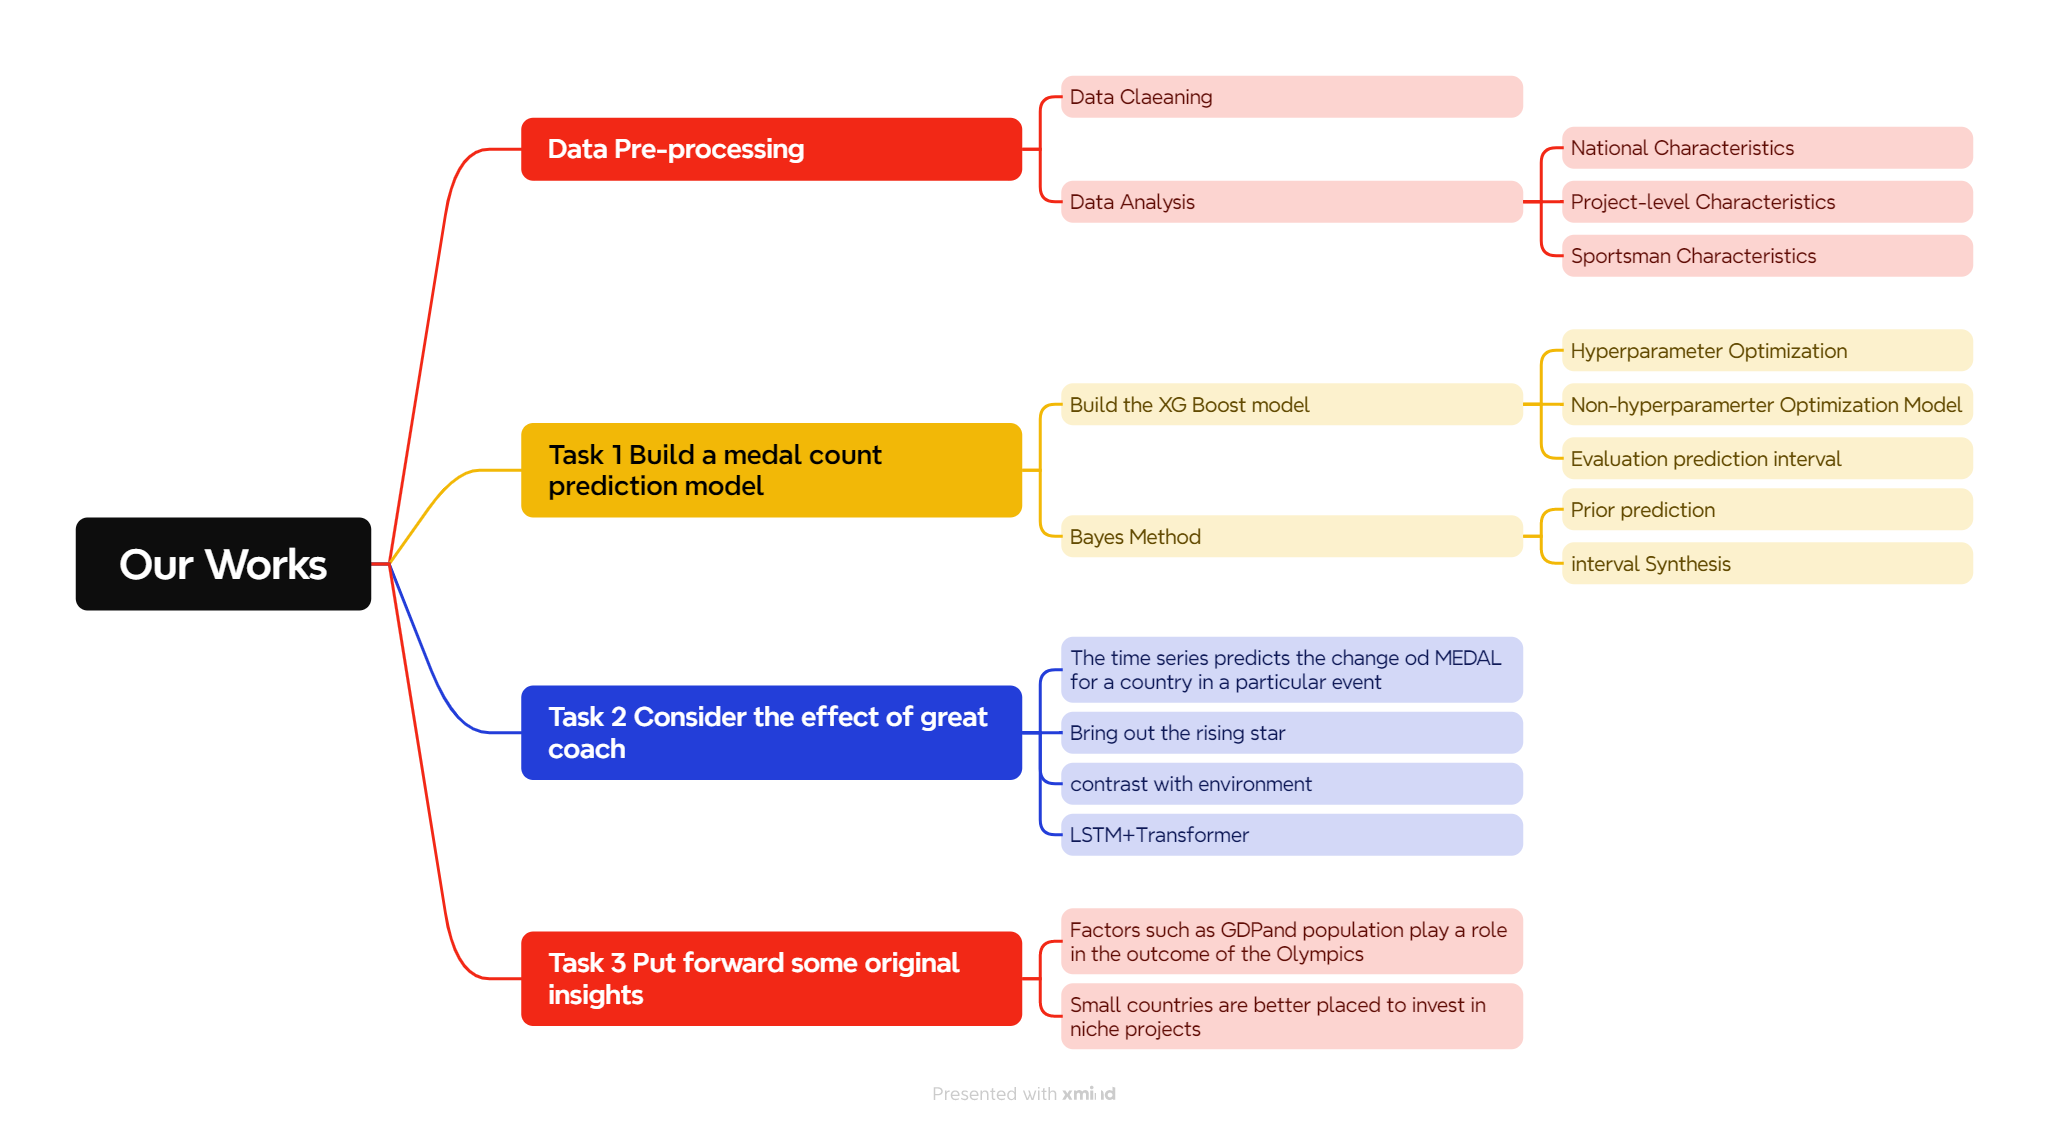
\includegraphics[width=0.5\textwidth]{figure/0.png} % 插入图片,宽度为文本宽度的一半
	\caption{1} % 图片标题
	\label{fig:example} % 图片标签,用于引用
\end{figure}

  \section{Model Preparation}
  \subsection{Assumptions}
  \begin{itemize}
    \item Assumption 1: The performance of athletes from each country in different sports is relatively stable.
    \item Assumption 2: The movement of coaches across countries significantly impacts the number of medals won.  
    \item Assumption 3: The choice of competition events greatly influences the medal distribution for the host country.
    \end{itemize}
    

  \subsection{Notations}
  The following notations are used throughout the paper:

  \begin{itemize}
      \item \( M_{i,t} \): Total number of medals won by country \( i \) in year \( t \).
      \item \( G_{i,t} \): Number of gold medals won by country \( i \) in year \( t \).
      \item \( S_{i,t} \): Number of silver medals won by country \( i \) in year \( t \).
      \item \( B_{i,t} \): Number of bronze medals won by country \( i \) in year \( t \).
      \item \( \Delta M_{i,t} \): Change in the total number of medals for country \( i \) from year \( t-1 \) to year \( t \).
      \item \( \Delta G_{i,t} \): Change in the number of gold medals for country \( i \) from year \( t-1 \) to year \( t \).
      \item \( NOC_i \): National Olympic Committee code for country \( i \).
      \item \( GDP_i \): Gross Domestic Product (GDP) of country \( i \).
      \item \( Pop_i \): Population of country \( i \).
      \item \( C_i \): Number of great coaches in country \( i \).
      \item \( X_{i,t} \): Feature vector for country \( i \) in year \( t \), including historical medal counts, GDP, population, and other socio-economic factors.
      \item \( \hat{M}_{i,t} \): Predicted total number of medals for country \( i \) in year \( t \).
      \item \( \hat{G}_{i,t} \): Predicted number of gold medals for country \( i \) in year \( t \).
      \item \( \epsilon \): Error term in the prediction model.
      \item \( \theta \): Model parameters to be optimized.
      \item \( AUC \): Area Under the Curve, used to evaluate the performance of classification models.
      \item \( MSE \): Mean Squared Error, used to evaluate the performance of regression models.
      \item \( \alpha \): Learning rate in machine learning models.
      \item \( \beta \): Regularization parameter in machine learning models.
      \item \( \gamma \): Threshold for determining progress, regression, or stability in medal counts.
      \item \( \sigma \): Standard deviation of the prediction interval.
  \end{itemize}
  
  \subsection*{Explanation of Notations}
  \begin{itemize}
      \item \textbf{Medal Counts}: \( M_{i,t} \), \( G_{i,t} \), \( S_{i,t} \), and \( B_{i,t} \) represent the total number of medals, gold medals, silver medals, and bronze medals won by country \( i \) in year \( t \), respectively.
      \item \textbf{Change in Medals}: \( \Delta M_{i,t} \) and \( \Delta G_{i,t} \) represent the change in the total number of medals and gold medals from the previous year, used to determine progress or regression.
      \item \textbf{Socio-Economic Factors}: \( GDP_i \) and \( Pop_i \) are used as features in the prediction model to account for the economic and demographic factors that may influence a country's performance in the Olympics.
      \item \textbf{Prediction Variables}: \( \hat{M}_{i,t} \) and \( \hat{G}_{i,t} \) represent the predicted number of total medals and gold medals for country \( i \) in year \( t \), respectively.
      \item \textbf{Model Evaluation Metrics}: \( AUC \) and \( MSE \) are used to evaluate the performance of the prediction models.
  \end{itemize}
 

  \section{Data Cleaning}
  \subsection{Missing Values}
  We found that only the program file had data missing.
  \subsection{Complete Outliers }
  We found missing data, with some of the missing values caused by changes in the rules of the competition in certain years. For example, the inclusion of ice skating events in the Winter Olympics led to missing data. We set the missing values for this part of the data to 0, while the remaining missing data was imputed using Random Forest, KNN and linear regression.
  \subsection{Perform Data Cleaning}
  \begin{itemize}
    \item Clean and organize Olympic medal data.
    \item Converts the data into a table form with the year as the column and the country as the row.
    \item Save the sorted data as a CSV file and output some results.
    \end{itemize}
    \subsection{Clean Outliers}
    We perform data preprocessing and identify outliers. For instance, the medal count of the United States is unusually high around World War I and World War II. The first step is to use Cook’s Distance to detect large deviations and identify potential outliers. The second step involves using KNN and multiple linear regression to impute the outliers. Finally, we create visualizations to check whether the adjustments have been successfully made.
    \subsection{State Transitions}
We define a country name mapping relationship , which is used to unify different forms of country names into standard names. Remove the countries that do not exist today, keep the countries that do exist today, and combine the countries to take the average.
\subsection{Convert the Format}
\begin{itemize}
  \item Convert Olympic athlete data from a long format to a wide format for easy analysis and visualization.
  \item Clean data and fill in missing values.
  \item Save the converted data as a CSV file.
  \end{itemize}

  \section{Data Analysis}
  \subsection{National Characteristics}
  The national characteristic value mainly includes the total number of historical MEDALS, the number of gold MEDALS and the growth rate of MEDALS.
  Due to the complexity of the data format, it is necessary to convert it to a more manageable format first, extract the year and the total number of MEDALS of each country, assuming that we focus on the total number of MEDALS of the United States and China, and finally draw a line chart to show the change trend of the total number of MEDALS of the two countries.
  \subsection{Project-level Characteristics}
  \subsection{Sportsman Characteristics}
  \subsubsection{Data preprocessing}
  We extracted the necessary columns, merged the Name,Sex,NOC columns, and sorted each athlete.
  \subsubsection{Add Unique Eigenvalues}
  Firstly, we discovered that in the provided data, there were cases where athletes participated again after a long interval of time, and there were also cases where athletes' names, genders, nationalities, and events were exactly the same but their ages differed by more than 100 years. Therefore, we made the following regulations: if the time interval is over 44 years, it will be automatically judged as different individuals. Secondly, regarding the issue of whether the participants who participated within a time interval of less than 44 years are the same, we used the DBSCAN algorithm for cluster analysis. Finally, we added feature values to distinguish athletes.
  \subsubsection{Count consecutive Olympic years and participant numbers.}
  The result is shown in the figure.

  
  


 
  
  \subsubsection{Participation Duration.}
  The result is shown in the figure.
 
  According to the fan chart, for athletes participating in consecutive competitions, only the continuous effects of athletes participating in 2-3 consecutive sessions are considered, and the remaining effects are negligible.
  We then calculate the proportion of athletes who participated continuously for a time span of 0-15 years. The discovery ratio was 94.51\%.
  The result is shown in the figure.
  \subsubsection{Some Conclusions}
  \begin{itemize}
    \item Most of the athletes who participate in the Olympic Games in the span of 0-15 years are continuous participation.
    \item Most of the athletes' time span is between 0-15 years, and the number of consecutive participation is 1-3 years.
    \item Most Olympic athletes have participated in 1-3 consecutive Olympic Games.
    \item To consider the impact of an athlete's consecutive participation on MEDALS, it is only necessary to consider the case of two or three consecutive entries.
    \end{itemize}
    The result is shown in the figure.
\begin{table}[h!]
  \centering
  \caption{probability of Athletes Participating in the Next Olympics Based On Previous Participations}
   
  \label{tab:olympic participation}
   \begin{tabular}{|c|c|}
    \hline
    \textbf{Number of Participation} & \textbf{Probability of Next Participation(\%)}\\
\hline
1&16.80\\
\hline
2&19.03\\
\hline
3&25.86\\
\hline
   \end{tabular}
  \end{table}
    \section{Task 1: Build a medal count prediction model}
 \subsection{Build the XG Boost model} 
 \subsubsection{Direct Prediction (Hyperparameter Optimization)} 
 The country code is first labeled and the missing values are processed. Features are then created, including the total number of MEDALS, gold, silver and bronze MEDALS from the previous year. The model is then built with XGBoostRegressor and the hyperparameters are optimized with GridSearchCV. Subsequently, the training set and test set are divided, the model is trained and the performance is evaluated, using the mean square error (MSE) as the evaluation metric. The model is trained individually for each country and weighted predictions are made in conjunction with the global model. Finally, predict the number of MEDALS won at the 2020 Olympics and save the results as a CSV file.
 \subsubsection{Non-hyperparameter Optimization Model} 
 First, the country code is labeled and the missing values are processed. Features are then created, including the total number of MEDALS, gold, silver and bronze MEDALS from the previous year. Next, build models with XGBoost Regressor and optimize hyperparameters with GridSearchCV. Subsequently, the training set and test set are divided, the model is trained and the performance is evaluated, using the mean square error (MSE) as the evaluation metric. The model is trained individually for each country and weighted predictions are made in conjunction with the global model. Finally, predict the number of MEDALS won at the 2020 Olympics and save the results as a CSV file.
 \subsubsection{Evaluation prediction interval.} 
 First, the Olympic medal data is imported and the country codes are labeled, while missing values are processed. Next, you define features and labels, and use XGBoost to build and train a classification model. For prediction, a function is defined to compute the prediction interval and applied to the data set. Finally, the code saves the prediction results and calculates the AUC evaluation metrics for the model. This code shows how to use the XGBoost model for data processing, training, and prediction, and to calculate prediction intervals and AUC evaluation metrics.
 \subsection{Bayes Method} 
 \subsubsection{Prior Prediction} 
 First, the Olympic medal data is loaded from the CSV file. The country code is encoded, missing values are processed, and features (such as the number of medals from the previous year) are created. Then, the posterior mean and standard deviation of the private and global forecasts are calculated using the Bayesian update formula, and the comprehensive forecast results are weighted according to the data volume. Next, XGBoost regression models are constructed to predict the total number of medals, gold medals, silver medals, and bronze medals, with hyperparameter optimization using GridSearchCV. Finally, model performance is evaluated, each country's model is trained individually, weighted predictions are made combining the global model, and the prediction results are saved as CSV files.
 \subsubsection{Interval Synthesis} 
 We calculate the mean, maximum, and minimum values based on NOC columns by merging databases.
 \section{Solving the First Given Problem} 
 \subsection{Problem 1: The country progresses or regresses} 
 We calculate the proportion of Total Change and Gold Change relative to Total change and Gold change to determine whether it is progress, regression, or stability.
 \begin{itemize}
  \item  Progress (Front) : Change is greater than 15\%.
  \item Back: The percentage change is less than -15\%.
  \item Stable: The percentage of change is between -15\% and 15\%.
  \item Special cases:
  
  If Total or Gold is 0, progress or stability is judged directly on the positive or negative of Total Change or Gold Change.
 
  If Total Change or Gold Change is 0, it is marked as stable.
  \end{itemize}
  \subsection{Problem 2: National First Prize Prediction} 
  \subsubsection{Data preprocessing} 
  \begin{itemize}
    \item Pre-processing: Load the data with Pandas, clean the country name (NOC) with regular expressions, and keep only English characters.
    \item Feature extraction: Traverse the data to record the year in which each country first won any medal or gold medal.
    \item Aggregate statistics: The number of first time winners/gold winners according to the actual Olympic year.
    \item Visualization: Matplotlib draws double line plots to compare historical trends. The process includes data cleaning, dictionary mapping, time series statistics and visualization.
  \end{itemize}
  \subsubsection{Linear Regression Prediction} 
We then ran linear regression projections to predict the number of countries that will win gold MEDALS for the first time in 2028.
  
  Tu
  
  Then we analyze the effects and calculate the fit of the model. The fit of the model for the number of countries winning gold MEDALS for the first time (Coefficient of Determination): 0.02
  
  Number of countries winning MEDALS for the first time: 43.33\% Number of countries winning gold for the first time: 33.33\%
  \subsubsection{ Evaluate the Possibility} 
 We train the linear regression model to predict the 2028 value, and calculate the confidence interval using the stats models.
 \subsection{Problem 3: Event and National Impact} 
 \subsubsection{Advantageous Projects by Country}
 We do the preprocessing first, defining a function that converts the value in the Medal column to the corresponding medal type, ensuring that the medal column is a numeric type. A function is then defined to obtain the top 2 sports in each country's overall medal tally and gold medal tally to derive the dominant events.
 \subsubsection{Host Effect}
 We first conducted a regression analysis model by creating a host identifier variable and selecting relevant features and target variables. The data were standardized, and a constant term was incorporated to construct the regression model. Finally, the mean coefficient of the Is Host variable was calculated. The results revealed that this coefficient was significantly positive, indicating that serving as the host nation exerts a statistically meaningful positive impact on the total medal count.
 \section{Task 2: Consider the effect of great coaches. } 
 We utilize time series forecasting to analyze medal count variations in specific events for a target nation. We utilize the LSTM+Transformer model. When significant deviations from predicted trends are observed—particularly years exhibiting anomalous upward trends—these instances are systematically flagged. By cross-referencing such anomalies with the baseline conditions defined in Environment I, the presence of the "Great Coach Effect" can be identified, thereby quantifying the impact of exceptional coaching interventions on performance outcomes.
 \section{Task 3: Put forward some original insights. } 
 \begin{itemize}
  \item Pre-processing: Load the data with Pandas, clean the country name (NOC) with regular expressions, and keep only English characters.
  \item Feature extraction: Traverse the data to record the year in which each country first won any medal or gold medal.
  \item Aggregate statistics: The number of first time winners/gold winners according to the actual Olympic year.
  \item Visualization: Matplotlib draws double line plots to compare historical trends. The process includes data cleaning, dictionary mapping, time series statistics and visualization.
\end{itemize}
\section{Strengths \&amp; Weaknesses} 
\subsection{ Strengths}
\begin{enumerate}
    \item \textbf{Superior Model:} The [Model Name] used outperforms traditional methods in accuracy and performance. It can handle single data points and full data series, fitting well for complex time - series datasets and task [Task Number] challenges.
    \item \textbf{Task - Result Consistency:} Results from task [Task Number 1] and task [Task Number 2] are highly congruent, proving the model's accuracy and reliability. Specific findings from each task mutually validate key insights.
    \item \textbf{Robust Data Methodology:} The model adopts a rigorous data - driven approach. Thorough data collection, cleaning, pre - processing, and feature engineering help it capture data patterns, ensuring superior performance.
\end{enumerate}
\subsection{Weaknesses}
\begin{enumerate}
    \item \textbf{Linear Regression Limitation:} The linear regression model exhibits poor fit, with an $R^{2}$ of only 0.02 for predicting first - time gold - winning countries, indicating its unsuitability for non - linear problems.
    \item \textbf{Athlete Feature Omission:} The model relies on national - level data (medal totals, GDP, population) but neglects athlete - specific features (age, training duration, injury status), which may significantly affect medal distribution.
    \item \textbf{Long - Term Validation Absence:} Focused on the 2028 Los Angeles Olympics, the model's long - term predictive ability (e.g., for 2032 or beyond) is unvalidated, with long - term forecasts subject to more uncertainties.
    \item \textbf{High Computational Cost \& Poor Hardware Utilization:}Training XGBoost hyper - parameter optimization and Transformer models takes >20 mins on a full - loaded 14900HX. A decision - tree count of 100 - 300 makes 4090 GPU less efficient than the 14900 due to data - transfer overheads. Model and parameter optimization is needed.
  \end{enumerate}

\subsection{Model Generalization}
\begin{enumerate}
    \item \textbf{Multi - event Adaptability:} The model can be extended to other international sports events (e.g., Winter Olympics, Asian Games, World Championships). By tuning variables like event types and participant numbers, it assesses medal - distribution patterns.
    \item \textbf{Variable Augmentation:} Integrating extra external data (e.g., education spend, sports facility building) can optimize prediction and uncover more influencing factors.
    \item \textbf{Real - time Prediction:} The model is integrable into real - time systems, updating medal forecasts dynamically during the Olympics for real - time decision support.
\end{enumerate}
\section{Summary}
This paper focuses on predicting the medal distribution of the 2028 Los Angeles Olympics. Given the Olympics' global significance and the medal table's role in reflecting national athletic strength, accurate prediction is crucial.

In data processing, rigorous cleaning and pre - processing were carried out. Missing values in the program file were handled using a combination of methods, and outliers in the medal file were detected and adjusted. Country names were standardized, and athlete data was formatted for analysis, ensuring data quality.

The model integrates XGBoost, Bayesian methods, and linear regression. Hyperparameters of XGBoost were optimized with GridSearchCV. Bayesian methods enabled probabilistic forecasts, and linear regression was used for specific predictions like first - time gold - medal - winning countries in 2028.

This integrated approach has notable strengths. It considers multiple factors such as historical medal data, socio - economic indicators, and coaching influence. By combining models, it provides weighted and probabilistic predictions, enhancing accuracy and reliability.

In conclusion, this research offers valuable contributions to Olympic medal prediction. It presents a new perspective and a practical model for relevant stakeholders. Future work can focus on model optimization and broader application exploration.






\begin{thebibliography}{99}
\bibitem{1} Hochreiter, S., \& Schmidhuber, J. (1997). LSTM. Neural Computation, 9(8), 1735-1780.
\bibitem{2}Hanley, J., \& Linder, D. (2017). Using Random Forests for Olympic Medal Prediction. Journal of Sports Analytics, 3(4), 145-156.
\bibitem{3}Cortes, C., \& Vapnik, V. (1995). Support vector networks. Machine Learning, 20(3), 273-297.
\bibitem{4}Gelman, A., et al. (2013). Bayesian Data Analysis (3rd ed.). CRC Press.
\bibitem{5}Metropolis, N., \& Ulam, S. (1949). The Monte Carlo method. Journal of the American Statistical Association, 44(247), 335-341.
\bibitem{6}Li, Z., \& Chen, J. (2020). The influence of coaching leadership on Olympic medal counts. International Journal of Sport Science and Coaching, 15(2), 298-310.
\end{thebibliography}

\begin{appendices}

%  备忘录正文部分
%  \begin{memo}[Memorandum]
% 	\lipsum[1-3]
% \end{memo}

\section{First appendix}

\lipsum[13]

Here are simulation programmes we used in our model as follow.\\

\textbf{\textcolor[rgb]{0.98,0.00,0.00}{Input matlab source:}}
\lstinputlisting[language=Matlab]{./code/mcmthesis-matlab1.m}

\section{Second appendix}

some more text \textcolor[rgb]{0.98,0.00,0.00}{\textbf{Input C++ source:}}
\lstinputlisting[language=C++]{./code/mcmthesis-sudoku.cpp}

\end{appendices}
\end{document}

%% 
%% This work consists of these files mcmthesis.dtx,
%%                                   figures/ and
%%                                   code/,
%% and the derived files             mcmthesis.cls,
%%                                   mcmthesis-demo.tex,
%%                                   README,
%%                                   LICENSE,
%%                                   mcmthesis.pdf and
%%                                   mcmthesis-demo.pdf.
%%
%% End of file `mcmthesis-demo.tex'.
